\section{movable  Class Reference}
\label{classmovable}\index{movable@{movable}}
Mostly virtual class for any entity in the scene. 


{\tt \#include $<$movable.hpp$>$}

Inheritance diagram for movable::\begin{figure}[H]
\begin{center}
\leavevmode
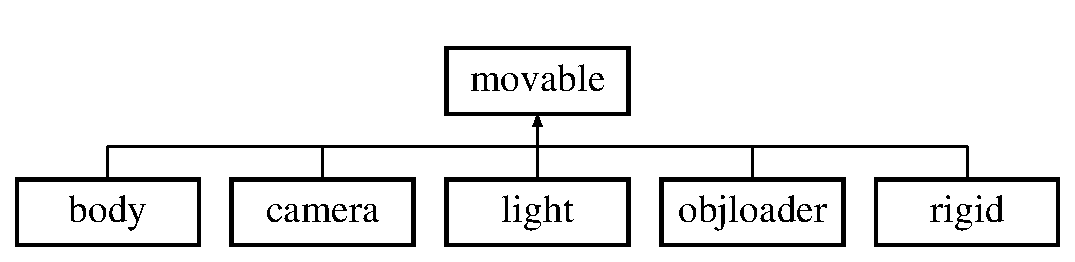
\includegraphics[height=2cm]{classmovable}
\end{center}
\end{figure}
\subsection*{Public Methods}
\begin{CompactItemize}
\item 
\index{movable@{movable}!movable@{movable}}\index{movable@{movable}!movable@{movable}}
{\bf movable} ()\label{classmovable_a0}

\item 
\index{movable@{movable}!movable@{movable}}\index{movable@{movable}!movable@{movable}}
{\bf movable} (string name)\label{classmovable_a1}

\item 
\index{~movable@{$\sim$movable}!movable@{movable}}\index{movable@{movable}!~movable@{$\sim$movable}}
virtual {\bf $\sim$movable} ()\label{classmovable_a2}

\item 
\index{init@{init}!movable@{movable}}\index{movable@{movable}!init@{init}}
void {\bf init} ()\label{classmovable_a3}

\item 
\index{operator=@{operator=}!movable@{movable}}\index{movable@{movable}!operator=@{operator=}}
movable \& {\bf operator=} (const movable \&other)\label{classmovable_a4}

\item 
\index{draw@{draw}!movable@{movable}}\index{movable@{movable}!draw@{draw}}
virtual void {\bf draw} ()\label{classmovable_a5}

\item 
\index{update@{update}!movable@{movable}}\index{movable@{movable}!update@{update}}
virtual void {\bf update} ()\label{classmovable_a6}

\item 
\index{move@{move}!movable@{movable}}\index{movable@{movable}!move@{move}}
void {\bf move} (int pitch, int turn, int roll, float x, float y, float z)\label{classmovable_a7}

\item 
\index{setName@{setName}!movable@{movable}}\index{movable@{movable}!setName@{set\-Name}}
void {\bf set\-Name} (string name)\label{classmovable_a8}

\item 
\index{getBoundingBox@{getBoundingBox}!movable@{movable}}\index{movable@{movable}!getBoundingBox@{get\-Bounding\-Box}}
virtual void {\bf get\-Bounding\-Box} ()\label{classmovable_a9}

\item 
\index{getAABB@{getAABB}!movable@{movable}}\index{movable@{movable}!getAABB@{get\-AABB}}
void {\bf get\-AABB} ()\label{classmovable_a10}

\item 
\index{drawAABB@{drawAABB}!movable@{movable}}\index{movable@{movable}!drawAABB@{draw\-AABB}}
void {\bf draw\-AABB} ()\label{classmovable_a11}

\item 
\index{drawBoundingBox@{drawBoundingBox}!movable@{movable}}\index{movable@{movable}!drawBoundingBox@{draw\-Bounding\-Box}}
void {\bf draw\-Bounding\-Box} ()\label{classmovable_a12}

\end{CompactItemize}
\subsection*{Public Attributes}
\begin{CompactItemize}
\item 
\index{mass@{mass}!movable@{movable}}\index{movable@{movable}!mass@{mass}}
float {\bf mass}\label{classmovable_m0}

\begin{CompactList}\small\item\em physical constants.\item\end{CompactList}\item 
\index{Ibody@{Ibody}!movable@{movable}}\index{movable@{movable}!Ibody@{Ibody}}
{\bf matrix9f} {\bf Ibody}\label{classmovable_m1}

\begin{CompactList}\small\item\em moment of inertia tensor.\item\end{CompactList}\item 
\index{IbodyInv@{IbodyInv}!movable@{movable}}\index{movable@{movable}!IbodyInv@{Ibody\-Inv}}
{\bf matrix9f} {\bf Ibody\-Inv}\label{classmovable_m2}

\begin{CompactList}\small\item\em inverse of moi tensor.\item\end{CompactList}\item 
\index{location@{location}!movable@{movable}}\index{movable@{movable}!location@{location}}
{\bf matrix16f} {\bf location}\label{classmovable_m3}

\begin{CompactList}\small\item\em state variable.\item\end{CompactList}\item 
\index{newLocation@{newLocation}!movable@{movable}}\index{movable@{movable}!newLocation@{new\-Location}}
{\bf matrix16f} {\bf new\-Location}\label{classmovable_m4}

\begin{CompactList}\small\item\em state variable.\item\end{CompactList}\item 
\index{P@{P}!movable@{movable}}\index{movable@{movable}!P@{P}}
{\bf vector3f} {\bf P}\label{classmovable_m5}

\begin{CompactList}\small\item\em momentum.\item\end{CompactList}\item 
\index{newP@{newP}!movable@{movable}}\index{movable@{movable}!newP@{new\-P}}
{\bf vector3f} {\bf new\-P}\label{classmovable_m6}

\begin{CompactList}\small\item\em momentum.\item\end{CompactList}\item 
\index{L@{L}!movable@{movable}}\index{movable@{movable}!L@{L}}
{\bf vector3f} {\bf L}\label{classmovable_m7}

\begin{CompactList}\small\item\em angular momentum.\item\end{CompactList}\item 
\index{newL@{newL}!movable@{movable}}\index{movable@{movable}!newL@{new\-L}}
{\bf vector3f} {\bf new\-L}\label{classmovable_m8}

\begin{CompactList}\small\item\em angular momentum.\item\end{CompactList}\item 
\index{Iinv@{Iinv}!movable@{movable}}\index{movable@{movable}!Iinv@{Iinv}}
{\bf matrix9f} {\bf Iinv}\label{classmovable_m9}

\item 
\index{velocity@{velocity}!movable@{movable}}\index{movable@{movable}!velocity@{velocity}}
{\bf vector3f} {\bf velocity}\label{classmovable_m10}

\begin{CompactList}\small\item\em velocity of center of mass.\item\end{CompactList}\item 
\index{omega@{omega}!movable@{movable}}\index{movable@{movable}!omega@{omega}}
{\bf vector3f} {\bf omega}\label{classmovable_m11}

\begin{CompactList}\small\item\em w angular velocity.\item\end{CompactList}\item 
\index{force@{force}!movable@{movable}}\index{movable@{movable}!force@{force}}
{\bf vector3f} {\bf force}\label{classmovable_m12}

\begin{CompactList}\small\item\em summed forces per timestep.\item\end{CompactList}\item 
\index{torque@{torque}!movable@{movable}}\index{movable@{movable}!torque@{torque}}
{\bf vector3f} {\bf torque}\label{classmovable_m13}

\begin{CompactList}\small\item\em summed torque per timestep.\item\end{CompactList}\item 
\index{normalize@{normalize}!movable@{movable}}\index{movable@{movable}!normalize@{normalize}}
bool {\bf normalize}\label{classmovable_m14}

\item 
\index{step@{step}!movable@{movable}}\index{movable@{movable}!step@{step}}
float {\bf step}\label{classmovable_m15}

\item 
\index{name@{name}!movable@{movable}}\index{movable@{movable}!name@{name}}
string {\bf name}\label{classmovable_m16}

\item 
\index{drawBB@{drawBB}!movable@{movable}}\index{movable@{movable}!drawBB@{draw\-BB}}
bool {\bf draw\-BB}\label{classmovable_m17}

\item 
\index{BBtested@{BBtested}!movable@{movable}}\index{movable@{movable}!BBtested@{BBtested}}
bool {\bf BBtested}\label{classmovable_m18}

\item 
\index{BBcollided@{BBcollided}!movable@{movable}}\index{movable@{movable}!BBcollided@{BBcollided}}
bool {\bf BBcollided}\label{classmovable_m19}

\item 
\index{centerBB@{centerBB}!movable@{movable}}\index{movable@{movable}!centerBB@{center\-BB}}
{\bf vector3f} {\bf center\-BB}\label{classmovable_m20}

\item 
\index{edgesBB@{edgesBB}!movable@{movable}}\index{movable@{movable}!edgesBB@{edges\-BB}}
{\bf vector3f} {\bf edges\-BB}\label{classmovable_m21}

\item 
\index{boundingBox@{boundingBox}!movable@{movable}}\index{movable@{movable}!boundingBox@{bounding\-Box}}
{\bf vector3f} {\bf bounding\-Box} [8]\label{classmovable_m22}

\item 
\index{oldCenterAABB@{oldCenterAABB}!movable@{movable}}\index{movable@{movable}!oldCenterAABB@{old\-Center\-AABB}}
{\bf vector3f} {\bf old\-Center\-AABB}\label{classmovable_m23}

\item 
\index{centerAABB@{centerAABB}!movable@{movable}}\index{movable@{movable}!centerAABB@{center\-AABB}}
{\bf vector3f} {\bf center\-AABB}\label{classmovable_m24}

\item 
\index{edgesAABB@{edgesAABB}!movable@{movable}}\index{movable@{movable}!edgesAABB@{edges\-AABB}}
{\bf vector3f} {\bf edges\-AABB}\label{classmovable_m25}

\item 
\index{AABB@{AABB}!movable@{movable}}\index{movable@{movable}!AABB@{AABB}}
{\bf vector3f} {\bf AABB} [8]\label{classmovable_m26}

\item 
\index{physical@{physical}!movable@{movable}}\index{movable@{movable}!physical@{physical}}
bool {\bf physical}\label{classmovable_m27}

\end{CompactItemize}


\subsection{Detailed Description}
Mostly virtual class for any entity in the scene.

It holds a lot of physical information that would be better off in a subclass where it would make sense, as lights and {\bf camera} {\rm (p.\,\pageref{classcamera})} don't really need such properties. 



The documentation for this class was generated from the following files:\begin{CompactItemize}
\item 
{\bf movable.hpp}\item 
movable.cpp\end{CompactItemize}
